
\indent \indent
After the optimization of the variables during cross validation phase of the experiment the network is retrained using all the available signal.  The remaining portion of the signal excluding the data for last 31 days is used to make the extended system states. These extended systems states and the computed $\textbf{W}^{out}$ is used to make prediction using Equation \ref{eq:prediction}. \\
There are 31 output neurons each of which makes the prediction for $n=1\hdots,31$ days ahead. The network optimized during cross validation phase and retrained afterwards us used to make the prediction for the number of views for the month of December 2016. The accuracy of each of prediction range is calculated as NRMSE. These error measures are plotted in the Figure \ref{fig:nrmsevspw}. The predicted number of views and the actual number of views for different prediction horizon are plotted in figure \ref{fig:realvspredicted}. As seen in Figure \ref{fig:nrmsevspw}, usually the NRMSE for the smaller prediction horizon is smaller. For longer prediction horizon the NRMSE is bigger. The NRMSE values doesn't increases linearly with the prediction horizon. One reason for this could be, I assume, that some of the features like biweekly repetition of triweekly correlation of the data might be strong that any other frequency.
\\
The optimizable parameters that worked best for this experiment are presented in the table \ref{table:optimized}.

	\begin{center}
	\captionof{table}{Optimized values for control parameters} \label{table:optimized} 
	\begin{tabular}{|c|c|c|} \hline
		 \multicolumn{2}{|l|}{ Parameters }& Optimized value\\ \hline
		 \multicolumn{2}{|l|}{ $sf^{\mathbf{W}}$}& 1.0\\ \hline
		 \multicolumn{2}{|l|}{$sf^{\mathbf{Win}}$}& 1.9 \\ \hline
		 \multicolumn{2}{|l|}{$sf^{\mathbf{B}}$}& 1.4\\ \hline
		  $\alpha$& HIGH& 5.05\\ \hline
		 \multicolumn{2}{|l|}{$sf_{sine}$} &\\ \hline
		 \multicolumn{2}{|l|}{ $sf_{add}$} &  \\ \hline
		 \multirow{3}{*}{$\alpha$} & FAST & \\ \cline{2-3}
		                   & MEDIUM &\\ \cline{2-3}
						   & SLOW &   \\\hline		 
	\end{tabular}
	\end{center}
	
	
  \begin{figure}[h]
     \centering
     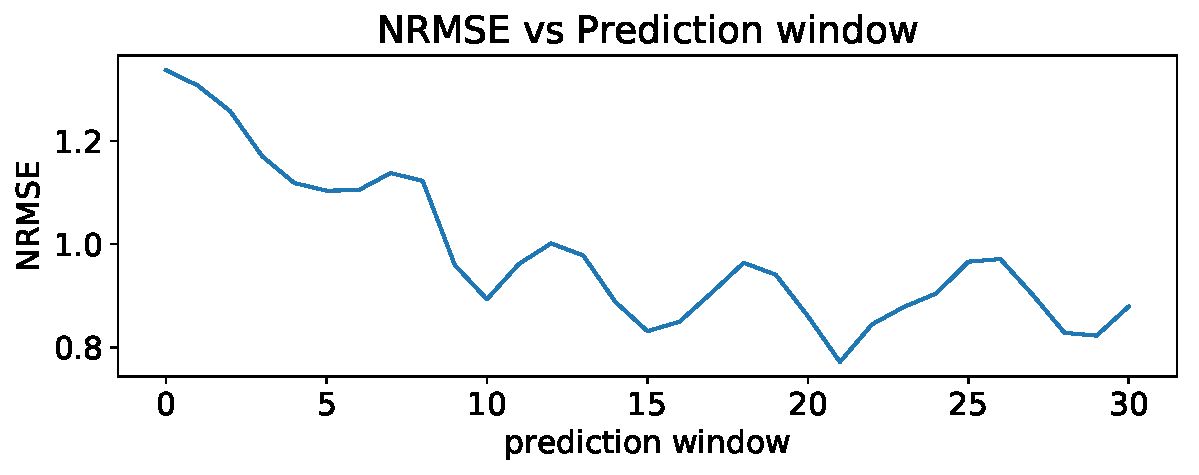
\includegraphics[width=\textwidth]{./results/images/nrmsevspwrec}

      \caption{NRMSE for different prediction window ranges}\label{fig:nrmsevspw}
  \end{figure}
 
 \begin{figure}[h]
    \centering
    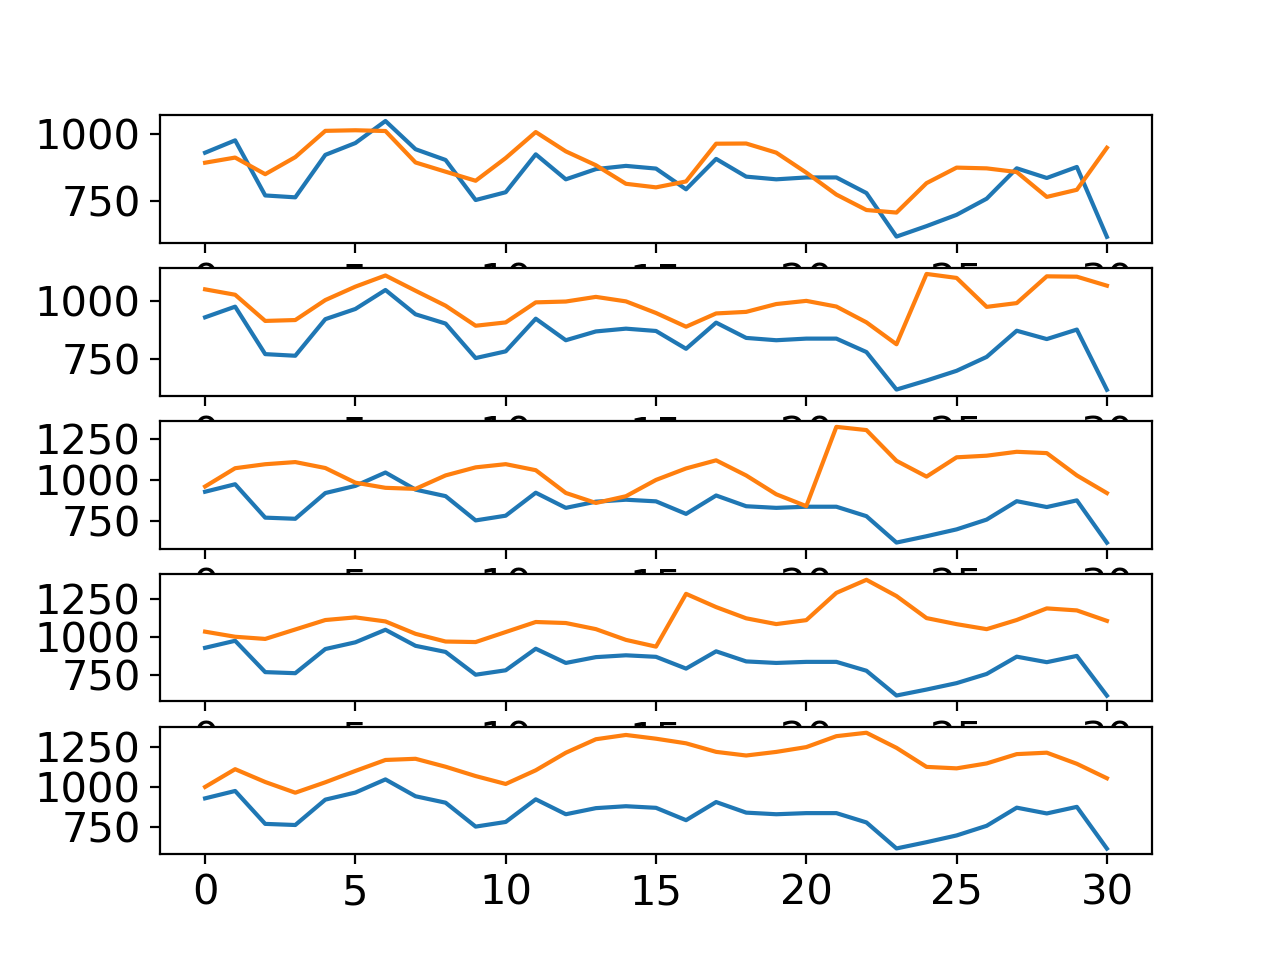
\includegraphics[width=\textwidth]{./results/images/realvspredicted}

     \caption{NRMSE for different prediction window ranges}\label{fig:realvspredicted}
 \end{figure}
 
 \subsection{Observation}
 During the process of tuning the parameters of the network it was observed that the data preprocessing affects the prediction by the network at higher extent than other factors. The reason for it, I beleive, is that the preprocessing steps followed scales down the outlier in the training signal and also scales up the previously hidden features in the signal. Adding an additional sine wave to the input signal also significantly improves the prediction.  This is signal that represents the view received by the wikipedia page as a weekly trend. Therefore on adding extra sine wave signal as the input, the network can easily identify this weekly pattern. However additional inputs, number of views for the related Wikipedia pages does not have signifincant impact on the prediction. This could be because these additional are highly correlated to the main input signal and thus does not provide much additional information to the network about the signal. During cross validation phase with the smaller values of regularization coefficient, $\beta$ it was observed that the predicted values in some of folds deviated highly from the real values and also from the mean values. This is because with very small regularization coefficent the output weights gets bigger thus even small peturbation in input signal lead to the strong perturbation in the prediction. The network gave best result when the scaling factors for $sf_W$ and $sf_Win$ are in the range of 0.5 - 1.5 and 0.3 - 0.6 despite the fact that the difference in the performace is barely noticable with any values assigned in that range. 
 
 
 